% This is samplepaper.tex, a sample chapter demonstrating the
% LLNCS macro package for Springer Computer Science proceedings;
% Version 2.21 of 2022/01/12
%
\documentclass[runningheads]{llncs}
%
\usepackage[T1]{fontenc}
% T1 fonts will be used to generate the final print and online PDFs,
% so please use T1 fonts in your manuscript whenever possible.
% Other font encondings may result in incorrect characters.


% tightlist command for lists without linebreak
\providecommand{\tightlist}{%
  \setlength{\itemsep}{0pt}\setlength{\parskip}{0pt}}


% Pandoc citation processing
%From Pandoc 3.1.8
% definitions for citeproc citations
\NewDocumentCommand\citeproctext{}{}
\NewDocumentCommand\citeproc{mm}{%
  \begingroup\def\citeproctext{#2}\cite{#1}\endgroup}
\makeatletter
 % allow citations to break across lines
 \let\@cite@ofmt\@firstofone
 % avoid brackets around text for \cite:
 \def\@biblabel#1{}
 \def\@cite#1#2{{#1\if@tempswa , #2\fi}}
\makeatother
\newlength{\cslhangindent}
\setlength{\cslhangindent}{1.5em}
\newlength{\csllabelwidth}
\setlength{\csllabelwidth}{3em}
\newenvironment{CSLReferences}[2] % #1 hanging-indent, #2 entry-spacing
 {\begin{list}{}{%
  \setlength{\itemindent}{0pt}
  \setlength{\leftmargin}{0pt}
  \setlength{\parsep}{0pt}
  % turn on hanging indent if param 1 is 1
  \ifodd #1
   \setlength{\leftmargin}{\cslhangindent}
   \setlength{\itemindent}{-1\cslhangindent}
  \fi
  % set entry spacing
  \setlength{\itemsep}{#2\baselineskip}}}
 {\end{list}}
\usepackage{calc}
\newcommand{\CSLBlock}[1]{#1\hfill\break}
\newcommand{\CSLLeftMargin}[1]{\parbox[t]{\csllabelwidth}{#1}}
\newcommand{\CSLRightInline}[1]{\parbox[t]{\linewidth - \csllabelwidth}{#1}\break}
\newcommand{\CSLIndent}[1]{\hspace{\cslhangindent}#1}

\usepackage{booktabs}
\usepackage{siunitx}
\usepackage{hyperref}
\hypersetup{colorlinks = TRUE,  urlcolor = blue, linkcolor = blue, citecolor = blue}

\usepackage{booktabs}
\usepackage{longtable}
\usepackage{array}
\usepackage{multirow}
\usepackage{wrapfig}
\usepackage{float}
\usepackage{colortbl}
\usepackage{pdflscape}
\usepackage{tabu}
\usepackage{threeparttable}
\usepackage{threeparttablex}
\usepackage[normalem]{ulem}
\usepackage{makecell}
\usepackage{xcolor}


\usepackage{graphicx}
% Used for displaying a sample figure. If possible, figure files should
% be included in EPS format.
%
% If you use the hyperref package, please uncomment the following two lines
% to display URLs in blue roman font according to Springer's eBook style:
\usepackage{hyperref}
\usepackage{color}
\renewcommand\UrlFont{\color{blue}\rmfamily}


\begin{document}


\title{biclaR: Estimating the socio-environmental impacts of car
substitution by bicycle and public transit using open tools}
%
\titlerunning{biclaR: SE impacts of car substitution by bicycle and
public transit}
% If the paper title is too long for the running head, you can set
% an abbreviated paper title here
%
\author{Rosa Félix\inst{1}\orcidID{0000-0002-5642-6006} \and Filipe
Moura\inst{1}\orcidID{0000-0001-7749-8490} \and Robin
Lovelace\inst{2}\orcidID{0000-0001-5679-6536}}


\authorrunning{R. Félix et al.}
% First names are abbreviated in the running head.
% If there are more than two authors, 'et al.' is used.
%

\institute{CERIS - Instituto Superior Técnico, University of Lisbon. Av
Rovisco Pais 1049-001 Lisboa, Portugal\\
\email{\href{mailto:rosamfelix@tecnico.ulisboa.pt}{\nolinkurl{rosamfelix@tecnico.ulisboa.pt}}}\\ \and Institute
for Transport Studies, University of Leeds. 34-40 University Rd, Leeds
LS2 9JT, UK}

\maketitle              % typeset the header of the contribution
%
\begin{abstract}
This paper estimates the potential for cycling combined with public
transit (PT) as a substitute for car trips in the Lisbon metropolitan
area and assesses its socio-environmental impacts using open data and
open source tools. A decision support tool that facilitates the design
and development of a metropolitan cycling network was developed
(\emph{biclaR}). The social and environmental impacts were assessed
using the \emph{HEAT for Cycling} and the \emph{HEAT as a Service}
tools. The impacts of shifting car trips to PT were also estimated and
monetized. The results indicate that 10\% of trips could be made by
bicycle + PT combination. Shifting to cycling for the first-and-last
mile stages can reduce annual CO\textsubscript{2}eq emissions from 3,000
tons/day, with benefits over 10 years of at least €125 million. For the
PT leg, the transfer from car avoids of up to 20,500 tons of
CO\textsubscript{2}eq emissions per year. This evidence can support
policymakers to prioritize interventions that reduce the reliance on
private motor vehicles.

\keywords{Active transport \and Intermodality \and First and last
mile \and Health economic assessment \and Environmental
impacts \and Open methods}

\end{abstract}

\section{Introduction}\label{introduction}

Combining public transportation (PT) and cycling for the first and last
mile in metropolitan areas can significantly replace private car trips
{[}1, 2{]}. This approach requires interventions and programs to make
bicycling more appealing, and the resulting public investments can have
significant social and environmental benefits.

According to the latest mobility survey conducted in 2018 {[}3{]}, the
LMA registered a total of 5.3 million daily trips, with only 0.5\% by
bicycle. Car modal share was 58.4\%, while PT accounted for 15.5\%. The
number of intra-municipal trips --- with origin and destination in the
same municipality --- amounts to 3.5 million trips. This exceeds the
number of inter-municipal trips (1.8 million trips), involving travel
between different municipalities. Cars and public transport are the most
used modes for intercity trips, with cars being the predominant choice
for all journeys.

To achieve the cycling targets set by the Portuguese national cycling
strategy for 2025 and 2030 (4\% and 10\%, respectively), the Lisbon's
Metropolitan Department of Transport introduced
\emph{biclaR}\footnote{See
  \href{https://biclar.tmlmobilidade.pt/}{biclar.tmlmobilidade.pt}.}, a
decision support tool that facilitates the design and development of a
metropolitan cycling network {[}4{]}.

\emph{biclaR} builds on the Propensity to Cycle Tool\footnote{See
  \href{https://www.pct.bike/}{pct.bike}.} (PCT), a web application and
research project funded by the UK's Department for Transport in 2015
which launched nationally in 2017 as part of the government's Cycling
and Walking Investment Strategy. The PCT initially used only
origin-destination data for commuting trips as the basis of estimates of
cycling potential at zone, route and route network levels {[}5{]}.
However, to the best of our knowledge, this is the first time that the
method has been integrated with public transport data using multi-modal
routing to estimate the potential and benefits of multi-stage cycling
and PT trips.

This paper estimates the potential for combining cycling and PT to
substitute car trips in the LMA. After presenting the methods used, it
assesses its socio-environmental impacts using open data and open-source
tools.

\section{Methods}\label{methods}

\subsection{Modeling Origin-Destination
trips}\label{modeling-origin-destination-trips}

The mobility survey data {[}3{]} is the basis for this project and
defines the baseline scenario. Despite being conducted in the
pre-pandemic period (2017), this dataset represents the most
comprehensive and up-to-date information on urban mobility in Portuguese
metropolitan areas (Lisbon and Porto).

We used a method for disaggregating the origins and destinations of
trips between the centroids of two districts (same as ``parish'') to
ensure that a district is not solely characterized by a single point of
origin and destination for its trips. The OD Jittering method breaks
down a single point (i.e., the centroid of an area) into multiple random
points on the existing and neighboring road network, using OpenStreetMap
as a reference {[}6{]}. Using the
\href{https://github.com/dabreegster/odjitter}{\texttt{odjitter} R
package}, we employed a maximum disaggregation level of 100 trips per
O-D pair for this project. Although this method provides a more
realistic representation of the trips undertaken compared to the
traditional approach, it does not fully align with the actual O-D pairs
of trips, which remain unknown due to data privacy regulations.

\subsection{Modeling routes}\label{modeling-routes}

The mobility survey collects the origin and destination of trips but
does not include the respective routes. Modeling the realistic cycling +
PT routes between OD pairs depends on assumptions regarding the
characteristics of the cycling and road networks and the location of
public transport interfaces.

The selected route choice algorithm was the
\href{https://ipeagit.github.io/r5r/}{\texttt{r5r} R package} {[}7{]},
which allows for great flexibility in configuring estimated route types.
\texttt{r5r} can calculate multi-modal routes using PT combined with
other modes. It enables the identification of the most direct or safest
cycling routes, using the Level of Traffic Stress\footnote{see
  \href{https://docs.conveyal.com/learn-more/traffic-stress}{docs.conveyal.com/learn-more/traffic-stress}.}
(LTS) scale. The routes were estimated for the base scenario for both
types of networks: \emph{direct} and \emph{safe}, using LTS 4 and LTS 3,
respectively.

The \texttt{r5r} model used the OpenStreetMap road network and the GTFS
metropolitan data aggregated and validated. This information is crucial
for an accurate PT trip and route estimation.

\subsection{Modeling intermodality}\label{modeling-intermodality}

The intermodality scenario considers trips combining PT and cycling for
the first and last legs. In a conservative approach, we have restricted
our analysis to the first and last legs with a combined length of up to
5 km (for instance: 1 km from origin to interface \emph{A} plus 4 km
from interface \emph{B} to destination) or up to 25 minutes on bike.
Furthermore, we have imposed restrictions on PT usage to include only
trips with no PT transfers, and up to 2 hours (120 min). Additionally,
we have only included PT modes that can easily accommodate bicycles,
such as trains, ferries, trams, and inter-municipal bus lines equipped
with bike racks (Figure \ref{fig:map1}). Figure \ref{fig:map2}
illustrates the resulting bicycle routes to access the main PT
interfaces in the LMA.

\begin{figure}[h]

{\centering 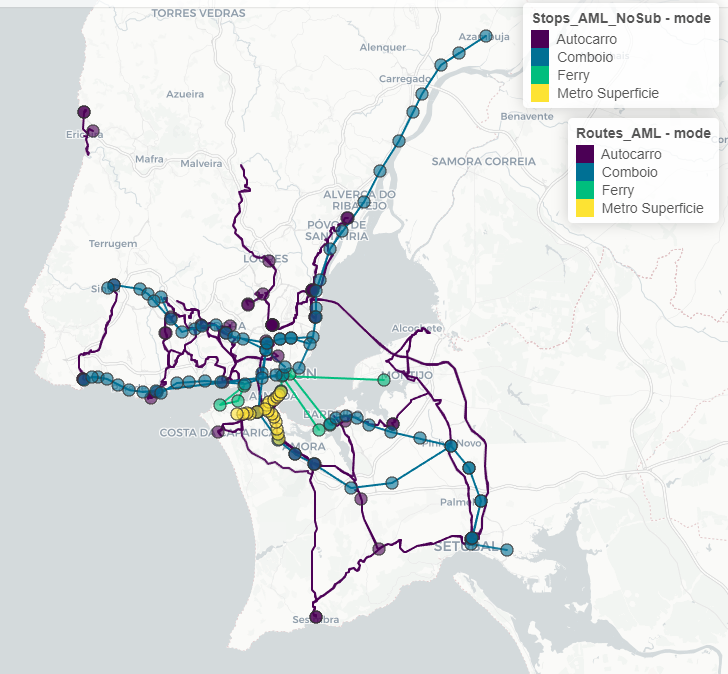
\includegraphics[width=0.6\linewidth,]{img/map1} 

}

\caption{Interfaces and lines considered, by transport mode, in the Lisbon metropolitan area. Author created map, using the mapview R package, with OpenStreetMap CARTO basemap.}\label{fig:map1}
\end{figure}

\begin{figure}[h]

{\centering 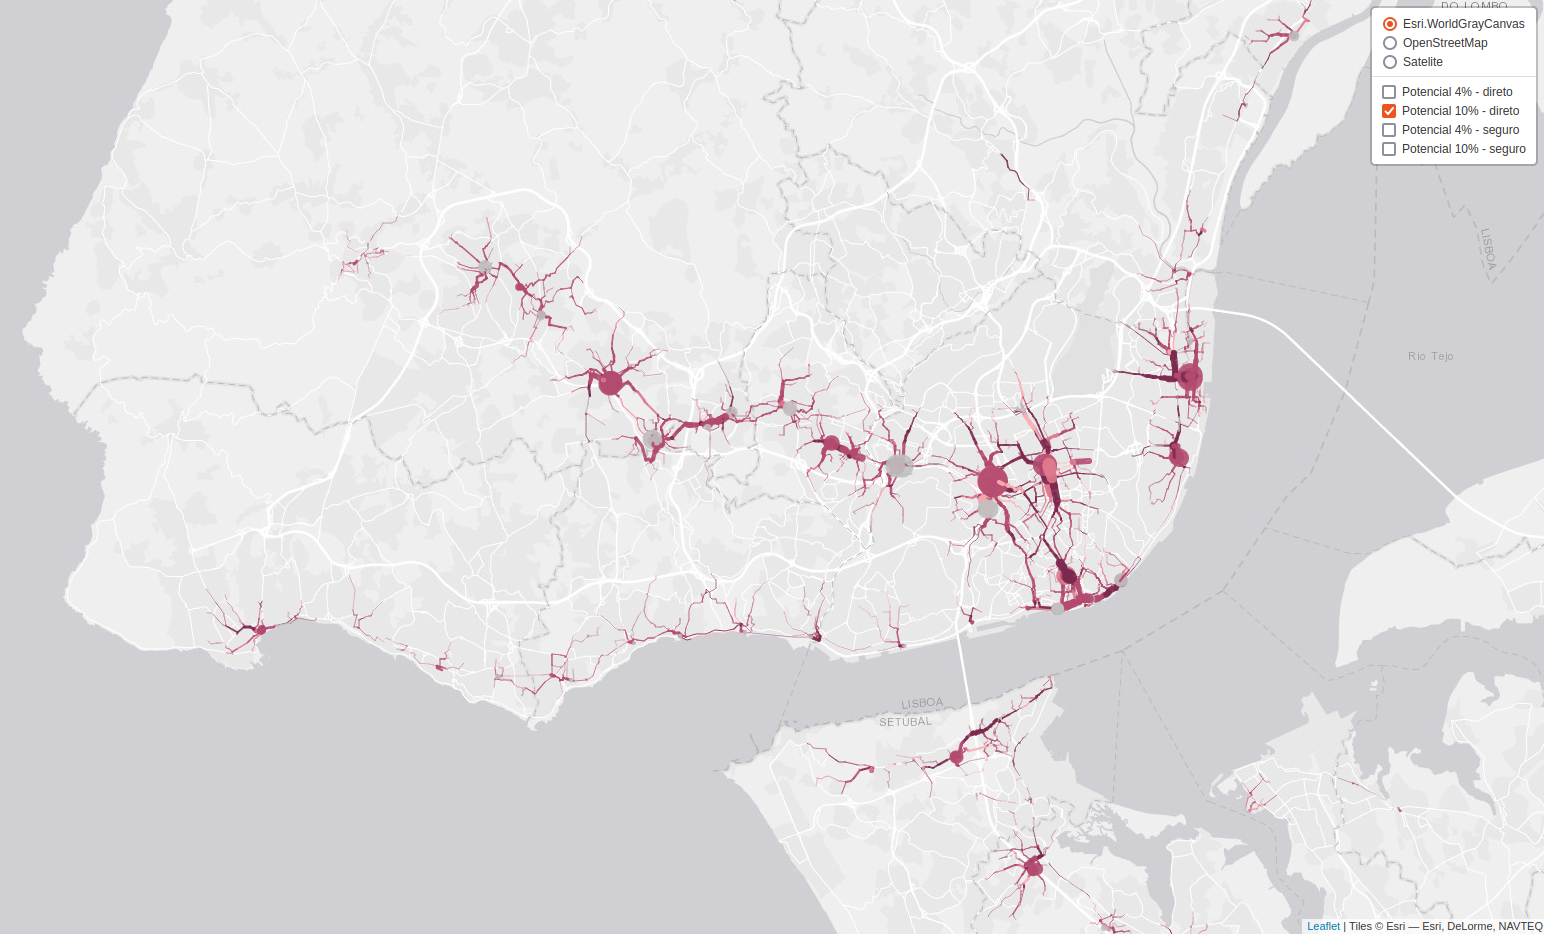
\includegraphics[width=0.8\linewidth,]{img/map2} 

}

\caption{Bike routes with highest potential to serve as first and last leg when replacing cycling and PT from car trips (screenshot of the interactive online tool).}\label{fig:map2}
\end{figure}

\subsection{Assessing socio-environmental
benefits}\label{assessing-socio-environmental-benefits}

For the cycling legs of the journey (first and last legs),
socio-environmental impacts were estimated on the shifting from car to
cycling, using the HEAT for Cycling tool v5.0 {[}8{]} from the World
Health Organization, and the
\href{https://github.com/HEAT-WHO/HEAT_heatr_api}{\texttt{HEATaaS} R
package}\footnote{\texttt{HEATaaS} is under development. For more
  information contact
  \href{https://heatwalkingcycling.org}{heatwalkingcycling.org}.}. We
considered two dimensions: \emph{social} --- including the physical
activity of cyclists, air pollution exposure, and road casualties;
\emph{environmental} --- including CO\textsubscript{2}eq emissions and
other pollutants.

For the second leg of the journey, we estimate the additional
environmental impacts of shifting car trips to PT (between the PT
interfaces).

To estimate the car emissions, we used the EMEP/EEA's COPERT software v5
methods and reference values {[}9{]} for a Tier 3 detail level.
Regarding PT, we considered the emission factor values reported in the
environmental and sustainability reports of the PT operators in the LMA.
The conversion of avoided emissions into avoided welfare loss and
respective monetary valuation was based on the EU Guide to Cost-benefit
Analysis {[}10{]} and the best up-to-date reference values for the
various gases.

\section{Results and Discussion}\label{results-and-discussion}

Table \ref{tab:summary1} presents the LMA total daily trips that can be
made with cycling + TP combination (with the aforementioned
restrictions), the trips in the baseline scenario and corresponding new
trips to achieve the national strategy targets (4\% and 10\%), for
different route profiles. For the cycling legs of the journey (first and
last legs), the environmental avoided emissions and monetized
socio-environment (SE) benefits are also presented, resulting from
replacing car trips with cycling.

\begin{table}

\caption{\label{tab:summary1}\label{summary1}Summary of the cycling potencial of intermodality scenario and its socio-environmental benefits for the cycling legs.}
\centering
\begin{tabular}[t]{llr>{\raggedleft\arraybackslash}p{6em}>{\raggedleft\arraybackslash}p{6em}>{\raggedleft\arraybackslash}p{6em}>{\raggedleft\arraybackslash}p{6em}}
\toprule
Target & Routing & Total trips & Baseline Cycling + PT & Potencial Cycling + PT & Avoided CO2eq (ton/yr) & SE Benefits for 10 years (thousand €)\\
\midrule
4\% & safe & 538 514 & 2 312 & 20 385 & 2 958 & 115 780\\
4\% & direct & 500 880 & 2 274 & 18 944 & 3 004 & 113 030\\
10\% & safe & 538 514 & 2 312 & 52 323 & 7 590 & 297 510\\
10\% & direct & 500 880 & 2 274 & 48 609 & 7 694 & 289 290\\
\bottomrule
\end{tabular}
\end{table}

For both \emph{direct} and \emph{safe} route profiles, 10\% of the daily
trips have the potential to be made by a combination of PT and cycling
(up to 5 km on bike). This unveils the potential of cycling as a
complementary mode of PT, with the potential to uptake the number of PT
trips within the LMA area by as much as 6.3\% (in addition to the 825
thousand PT trips reported in the mobility survey).

Regarding the PT mode to replace the second leg of the journey, in
combination with cycling, trains offer the greatest potential for
substitution (88\%). When comparing the existing PT interfaces (Figure
\ref{fig:map1}) with the bike routes with highest potential to serve as
first and last legs (Figure \ref{fig:map2}) it becomes clear that the
Train interfaces are the ones that have the highest potential to attract
car-to-PT substituting trips, if their accessibility by bicycle is
improved to be safe.

Regarding the PT segment, the shift from private car usage would lead to
the mitigation of CO\textsubscript{2} equivalent emissions to 8,500 to
20,800 tons annually, valued in €1.4 million to €3.5 million yearly.

The sum of CO\textsubscript{2}eq avoided emissions from the potential
car trips shifted to bike (first-and-last legs) in combination with PT
(second leg) in the LMA is presented on Table \ref{tab:summaryall}, for
both national cycling strategy targets and routing profiles, and the
socio-environmental benefits monetized in €, for a 1-year and 10-year
time periods.

\begin{table}

\caption{\label{tab:summaryall}\label{summaryall}Summary of the avoided CO2eq emmissions (ton/year) and the estimated social and environmental benefits (monetized in thousand €) by replacing car trips with cycling in combination with PT.}
\centering
\begin{tabular}[t]{ll>{\raggedleft\arraybackslash}p{8em}>{\raggedleft\arraybackslash}p{8em}>{\raggedleft\arraybackslash}p{8em}}
\toprule
Target & Routing & Avoided CO2eq (tons) & SE Benefits 1yr (k€) & SE Benefits 10yrs (k€)\\
\midrule
4\% & safe & 11 551 & 14 380 & 127 534\\
4\% & direct & 11 706 & 14 135 & 125 016\\
10\% & safe & 28 217 & 36 861 & 325 814\\
10\% & direct & 28 487 & 35 905 & 318 062\\
\bottomrule
\end{tabular}
\end{table}

Shifting from car to cycling + PT can reduce annual
CO\textsubscript{2}eq emissions emissions by 11,500 to 28,500 tons per
year, and the 10-year socio-environmental benefits account for €125
million to €325 million, depending on the cycling targets

The environmental impacts represent less than 2\% of the
socio-environmental benefits (in value) from replacing car trips to
bicycle in first-and-last legs. For the PT segment, we did not estimate
the social impacts from substituting car trips, although its health
benefits would not be as high as shifting to cycling.

The emissions of CO\textsubscript{2}eq that are avoided during both the
initial and final journey segments account for about 74\% of the
emissions avoided during the PT segment. This finding, while expected --
due the zero cycling emissions, should not be overlooked when promoting
the PT use. Improving the safe accessibility to PT interfaces to
cyclists and providing bicycle-friendly amenities such as parking
facilities can potentially lead to a higher reduction in
CO\textsubscript{2}eq emissions, compared to a scenario where
individuals shift from car travel to car + PT combination.

Our findings show that cycling \emph{in combination} with PT could
replace 10\% of current LMA trips, with an additional 6\% of PT journeys
prone to further substitution, based on conservative assumptions.

\section{Conclusion}\label{conclusion}

The information on socio-economic benefits can support policy-makers in
prioritizing interventions to reduce the reliance on individual
motorized transportation, and to better communicate their decisions by
providing the expected avoided GHG and air pollutant emissions and the
monetized socio-economic benefits for short and long terms.

The information available at \emph{biclaR} tool -- an open access
website -- can be downloaded and used with any GIS software. This allows
users to, for example, gain insights into which potential cycling
connections have the highest socio-environmental impacts, quantified in
tons of avoided CO\textsubscript{2}eq emissions, or in long term social
benefits.

By making the research process publicly accessible in a code repository,
this research enables the replication of similar estimates for
socio-environmental impacts, resulting from a modal shift from car to
bicycle in combination with PT, in other metropolitan areas.

\subsubsection*{Acknowledgements.}\label{acknowledgements.}
\addcontentsline{toc}{subsubsection}{Acknowledgements.}

This research was funded by the Lisbon's Metropolitan Department of
Transport (TML - Transportes Metropolitanos de Lisboa, E.M.T., S.A.),
under the \emph{biclaR} Project. This work is part of the research
activity carried out at Civil Engineering Research and Innovation for
Sustainability (CERIS) and has been funded by Fundação para a Ciência e
a Tecnologia (FCT), Portugal in the framework of project
UIDB/04625/2020.

\section*{References}\label{references}
\addcontentsline{toc}{section}{References}

\phantomsection\label{refs}
\begin{CSLReferences}{0}{0}
\bibitem[\citeproctext]{ref-MARTENS2007326}
\CSLLeftMargin{1. }%
\CSLRightInline{Martens, K.: Promoting bike-and-ride: The dutch
experience. Transportation Research Part A: Policy and Practice. 41,
326--338 (2007).
https://doi.org/\href{https://doi.org/10.1016/j.tra.2006.09.010}{10.1016/j.tra.2006.09.010}.}

\bibitem[\citeproctext]{ref-RIETVELD200071}
\CSLLeftMargin{2. }%
\CSLRightInline{Rietveld, P.: The accessibility of railway stations: The
role of the bicycle in the netherlands. Transportation Research Part D:
Transport and Environment. 5, 71--75 (2000).
https://doi.org/\href{https://doi.org/10.1016/S1361-9209(99)00019-X}{10.1016/S1361-9209(99)00019-X}.}

\bibitem[\citeproctext]{ref-IMOB}
\CSLLeftMargin{3. }%
\CSLRightInline{INE:
\href{https://www.ine.pt/xportal/xmain?xpid=INE&xpgid=ine_publicacoes&PUBLICACOESpub_boui=349495406&PUBLICACOESmodo=2&xlang=pt}{Mobilidade
e funcionalidade do território nas {Áreas Metropolitanas do Porto e de
Lisboa}: 2017}. {Instituto National de Estatística}, Lisboa (2018).}

\bibitem[\citeproctext]{ref-felix2023}
\CSLLeftMargin{4. }%
\CSLRightInline{Félix, R., Lovelace, R., Moura, F.: {biclaR - Ferramenta
de apoio ao planeamento da rede ciclável na área metropolitana de
Lisboa}, \url{https://biclar.tmlmobilidade.pt}, (2022).}

\bibitem[\citeproctext]{ref-lovelace2017}
\CSLLeftMargin{5. }%
\CSLRightInline{Lovelace, R., Goodman, A., Aldred, R., Berkoff, N.,
Abbas, A., Woodcock, J.: The Propensity to Cycle Tool: An open source
online system for sustainable transport planning. Journal of Transport
and Land Use. 10, (2017).
https://doi.org/\href{https://doi.org/10.5198/jtlu.2016.862}{10.5198/jtlu.2016.862}.}

\bibitem[\citeproctext]{ref-Lovelace2022Jittering}
\CSLLeftMargin{6. }%
\CSLRightInline{Lovelace, R., Félix, R., Carlino, D.: Jittering: A
computationally efficient method for generating realistic route networks
from origin-destination data. Findings. (2022).
https://doi.org/\href{https://doi.org/10.32866/001c.33873}{10.32866/001c.33873}.}

\bibitem[\citeproctext]{ref-r5r}
\CSLLeftMargin{7. }%
\CSLRightInline{Pereira, R.H.M., Saraiva, M., Herszenhut, D., Braga,
C.K.V., Conway, M.W.: r5r: Rapid realistic routing on multimodal
transport networks with R5 in r. Findings. (2021).
https://doi.org/\href{https://doi.org/10.32866/001c.21262}{10.32866/001c.21262}.}

\bibitem[\citeproctext]{ref-HEAT}
\CSLLeftMargin{8. }%
\CSLRightInline{Kahlmeier, S., Götschi, T., Cavill, N., Castro
Fernandez, A., Brand, C., Rojas Rueda, D., Woodcock, J., Kelly, P.,
Lieb, C., Oja, P., others:
\href{https://www.euro.who.int/__data/assets/pdf_file/0010/352963/Heat.pdf}{Health
economic assessment tool ({HEAT}) for walking and for cycling: Methods
and user guide on physical activity, air pollution, injuries and carbon
impact assessments}. (2017).}

\bibitem[\citeproctext]{ref-COPERT}
\CSLLeftMargin{9. }%
\CSLRightInline{Ntziachristos, L., Samaras, Z.: {EMEP/EEA} air pollutant
emission inventory guidebook 2019,
\url{https://www.emisia.com/utilities/copert/documentation/}, (2020).}

\bibitem[\citeproctext]{ref-EuropeanCommission2014}
\CSLLeftMargin{10. }%
\CSLRightInline{Sartori, D., Catalano, G., Genco, M., Pancotti, C.,
Sirtori, E., Vignetti, S., Del Bo, C.:
\href{https://ec.europa.eu/regional_policy/sources/docgener/studies/pdf/cba_guide.pdf}{Guide
to cost-benefit analysis of investment projects. Economic apraisal tool
for cohesion policy 2014-2020}. {European Commission - Directorate
General for Regional and Urban Policy} (2014).}

\end{CSLReferences}

%
% ---- Bibliography ----



\end{document}
